\documentclass[12pt]{article}
\usepackage{geometry}
\geometry{left=1in,right=0.75in,top=1in,bottom=1in}
\usepackage{lastpage}
\usepackage{fancyhdr}
\usepackage{color}
\usepackage{longtable}
\usepackage{graphicx}
% \usepackage{hyperref}
\usepackage[hidelinks]{hyperref}
\usepackage{tabularx}
\usepackage{float}
\usepackage[toc,page,title,titletoc,header]{appendix}
\usepackage[font=small,labelfont=bf]{caption}
\usepackage{ifthen}
\usepackage{pgfplots}
\usepackage{amsmath,amssymb,amsthm}
\usepackage{graphicx}
\usepackage{xcolor}
\usepackage{fancyhdr}
\usepackage{pgfplots}

\usepackage{minted}
\usepackage{booktabs}
\usepackage{indentfirst}
\usepackage{multirow}
\usepackage{tikz}
\usepackage{graphicx}
\usetikzlibrary{positioning}

\newcommand{\Problem}{B}
\newcommand{\Team}{2122216}

\numberwithin{equation}{section}
\graphicspath{{figures/}}
\lhead{Team \Team}
\rhead{}
\cfoot{}

% \setlength{\parindent}{2em}
\setlength{\parskip}{0.5em}

\theoremstyle{definition}
\newtheorem{definition}{\noindent Assumption}

\pagestyle{fancy}
\rhead{Page \thepage\ of \pageref{LastPage}}

%
\begin{document}

\thispagestyle{empty}
\vspace*{-16ex}
\centerline{
	\begin{tabular}{*3{c}}
		\parbox[t]{0.3\linewidth}{
			\begin{center}\textbf{Problem Chosen} \\
				\Large \textcolor{red}{\Problem}
			\end{center}} &
		\parbox[t]{0.3\linewidth}{
			\begin{center}
				\textbf{2020\\ MCM/ICM\\ Summary Sheet}
			\end{center}} &
		\parbox[t]{0.3\linewidth}{
			\begin{center}
				\textbf{Team Control Number} \\
				\Large \textcolor{red}{\Team}
			\end{center}} \\
		\hline
	\end{tabular}
}

% Summary
\begin{center}
\Large\bf Title of you paper
\end{center}

From here, begin your summary

\begin{center}
    \textbf{Keywords:} Abstract, \LaTeX, English
\end{center}


% Table of Contents
\clearpage
\newpage
% \setcounter{page}{1}
\tableofcontents
\newpage


% Contents
\section{Introduction}\label{sec:intro}

\subsection{Problem Background}

The carbon cycle describes the process of the exchange of carbon throughout the geochemical cycle of the Earth, and is a vital component for life on the planet. One key component of this part of the process is the decomposition of plant material and woody fibers.

Some of the key agents in decomposing woody fibers are fungi. The authors of a recent research article on wood decomposition by fungi identified fungi traits that determine decomposition rates and also noted links between certain traits. In particular, the slow growing strains of fungi tend to be better able to survive and grow in the presence of environmental changes with respect to moisture and temperature, while the faster growing strains tend to be less robust to the same changes.

\subsection{Problem Restatement}
\begin{itemize}
\item Build a mathematical model that describes the breakdown of ground litter and woody fibers through fungal activity in the presence of multiple species of fungi.
\item In your model, incorporate the interactions between different species of fungi, which have different growth rates and different moisture tolerances.
\item Provide an analysis of the model and describe the interactions between the different types of fungi. The dynamics of the interactions should be characterized and described including both short- and long-term trends. Your analysis should examine the sensitivity to rapid fluctuations in the environment, and you should determine the overall impact of changing atmospheric trends to assess the impact of variation of local weather patterns.
\item Include predictions about the relative advantages and disadvantages for each species and combinations of species likely to persist, and do so for different environments including arid, semi-arid, temperate, arboreal, and tropical rain forests.
\item Describe how the diversity of fungal communities of a system impacts the overall efficiency of a system with respect to the breakdown of ground litter. Predict the importance and role of biodiversity in the presence of different degrees of variability in the local environment.
\end{itemize}
\subsection{Our Work}

\begin{figure}\caption{Work flow of our modelling}
    \begin{center}
        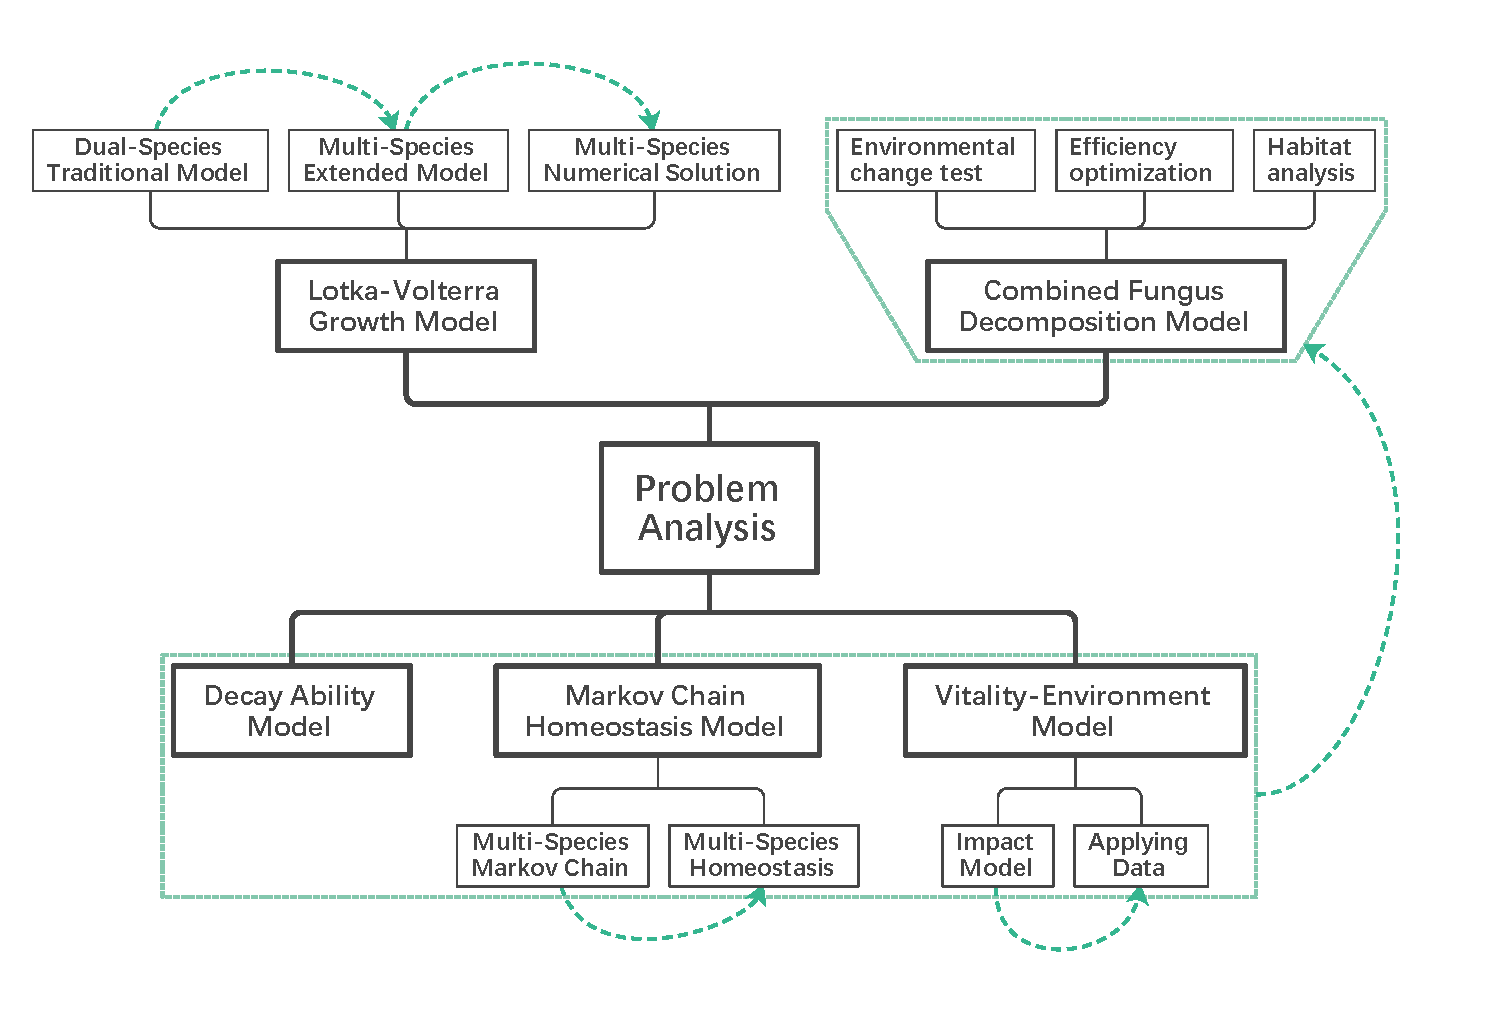
\includegraphics[width=\columnwidth]{workflow.pdf}
    \end{center}\end{figure}

\section{Assumptions and Notations}\label{sec:assump}

Our model is based on several approximate but reasonable assumptions. For a certain ecological configuration in restricted region, such as the decomposition process of a log dominated by fungus, it is equivalent for considering the quantity of fungus individual, biomass or population density. Therefore, our modeling is based on the population density of each species of fungus.

\paragraph{Assumption 1}: Under fixed environmental condition, the ability of a fungi population for decomposing ground litter and woody fibers is proportional to its population density, the coefficient of which is a constant.

\textbf{Justification}: The rate of decomposition is rather complicated, and with temporal memory, since it is in fact determined by the total amount of enzyme exists. In addition, two or more categories of enzyme may interact with each other or together to boost or resist the decomposition reaction. However, to simplify the problem, we ignore such mechanisms, and include all the other factors that affects the biological vitality of the fungus in a single parameter.

\paragraph{Assumption 2}: The constant mentioned above, hence the ability of different fungus species for decomposition, is only related to environmental temperature and humidity.

\textbf{Justification} According to the problem given and other researches, temperature and humidity are the two dominating factors for fungus community, and should be taken into consideration.

\paragraph{Assumption 3} The vital activity of fungus community, that is, the product of metabolization, has no effect on the environment humidity and temperature.

\textbf{Justification} In nature circumstances, the decomposition process happens in open air, the heat and moisture produced or absorbed by fungus can be promptly carried off or replenished  by the external environment, hence the local environment dominates the conditions of the growth of fungus community.

\paragraph{Assumption 4} The decomposition is dominated by the fungus community, and no other species have effect on the system.

\paragraph{Assumption 5} The inter-species relation among the populations in the community is merely competition.

\textbf{Justification} Other inter-species relations such as mutualism, parasitism and predation are rarely seen among fungus. Considering only competition enables us to utilize existed models.

\paragraph{}
Based on these assumptions, we defined the following notations in modeling.

\paragraph{}
\textbf{Assumption 3}: The

\textbf{Justification}: If

\begin{center}\begin{tabular}{ccc}
    \toprule
    Symbol & Definition & Unit \\
    \midrule
    a & b & c \\
    \bottomrule
\end{tabular}\end{center}
\section{Competition Model of the Growth of Fungus Community}\label{sec:LV}


\subsection{Lotka-Volterra Model for Dual-Species System}

In the early twentieth century, Alfred Lotka and Vito Volterra simultaneously derived a model that described how competition affects population growth from the perspective of differential equations, which is now known as the Lotka-Volterra, or LV model.

First, for single population, if the resources are sufficient enough, the population size, or similarly, density, is expected to grow in the form of

\begin{equation}\label{eq:exp}
    \frac{\mathrm{d}x_1}{\mathrm{d}t} = r_1x_1.
\end{equation}

In which, the intrinsic rate of increase $r$ is the per capita growth rate that could potentially be realized by a fungus population. However, unlimited growth is impossible in reality, environment itself has retardant effect on the population. Take the bounded carrying capacity into consideration, obtains

\begin{equation}\label{eq:logistic}
    \frac{\mathrm{d}x_1}{\mathrm{d}t} =
    r_1x_1\left(1 - \frac{x_1}{K_1}\right).
\end{equation}

The extra term places a limit on exponential growth, and the resulting equation represents the logistic growth.

In a dual-species system, the resistance against the growth of one population comes not only from the environment, but also another specie. It is natural that, when specie 2 has larger population density, specie 1 will be in face of larger competitive pressure, and similar for species 2. Such notion is also capable for intra-specie competition. Combining the inter-species and intr-specie competition into \eqref{eq:logistic}, obtains the differential equations set

\begin{equation}\label{eq:dual}
    \left\{\begin{aligned}     &
        \frac{\mathrm{d}x_1}{\mathrm{d}t} =
        r_1x_1\left(1 - \frac{\alpha_{11}x_1 + \alpha_{12}x_2}{K_1}\right) \\ &
        \frac{\mathrm{d}x_2}{\mathrm{d}t} =
        r_2x_2\left(1 - \frac{\alpha_{22}x_2 + \alpha_{21}x_1}{K_2}\right).
    \end{aligned}\right.
\end{equation}

Which is the model for dual-species competition. Note that, neither Lotka nor Volterra explained this equation from the perspective of ecology, it is Tilman who made a convincing interpretation. His resource-based model included resources requirement, consumption and supply, which is concise and rigorous but not the topic of this literature.


\subsection{Extended Lotka-Volterra Model for Multi-Species}

Based on LV model, we extended \eqref{eq:dual} to a multi-species system with $n$ various populations.

\begin{equation}\label{eq:dual}
    \left\{\begin{aligned}     &
    \frac{\mathrm{d}x_1}{\mathrm{d}t} =
    r_1x_1\left(1 - \frac{\sum_{j=1}^n \alpha_{1j}x_j}{K_1}\right) \\ & \cdots \\ &
    \frac{\mathrm{d}x_i}{\mathrm{d}t} =
    r_ix_i\left(1 - \frac{\sum_{j=1}^n \alpha_{ij}x_j}{K_i}\right) \\ & \cdots \\ &
    \frac{\mathrm{d}x_n}{\mathrm{d}t} =
    r_nx_n\left(1 - \frac{\sum_{j=1}^n \alpha_{nj}x_j}{K_n}\right)
    \end{aligned}\right.
\end{equation}

The equations set can be simplified with matrix differential equations as

\begin{equation}\label{eq:mat}
    \frac{\mathrm{d}\boldsymbol{x}}{\mathrm{d}t} =
    \boldsymbol{r}\cdot\boldsymbol{x}
    \left[\boldsymbol{1} - (\boldsymbol{Ax})\cdot\hat{\boldsymbol{K}}\right].
\end{equation}

In which the matrix $\hat{\boldsymbol{K}}$ is the element-wise reciprocal of $\boldsymbol{K}$, that is, $\hat{\boldsymbol{K}}_{ij}\boldsymbol{K}_{ij} = 1$. 

The growth process of fungus community considering competition is characterized by this first-order linear ordinary differential equations group, with $n$ unknown functions. Note that while the analytical can be difficult to be found, we can still figure out the development of the system using computer numerically.

Consider a quad-species system, with the parameters shown in table \ref{tb:quad-para}.

\begin{table}
    \begin{center}
        \caption{The parameters}
        \begin{tabular}{c|cccccc}
            \toprule
                  & $r_i$ & $K_i$ & $\alpha_{i1}$ & $\alpha_{i2}$ & $\alpha_{i3}$ & $\alpha_{i4}$ \\
            \midrule
            $x_1$ &       &       &               &               &               &               \\
            $x_2$ &       &       &               &               &               &               \\
            $x_3$ &       &       &               &               &               &               \\
            $x_4$ &       &       &               &               &               &               \\
            \bottomrule
        \end{tabular}\label{tb:quad-para}
    \end{center}
\end{table}

% TODO: Really that hard? Is there a solution?


% \subsection{Numerical}

\section{Homeostasis of the Community with Markov Chain Model}\label{sec:markov}


\subsection{Feasibility of utilizing Markov chain model in fungus community}

Since it is presumably impractical for finding the symbolic solution of the LV model, Markov chain model is introduced for predicting the stable state, that is, the relatively static composition of the fungus populations density in the community.

\begin{definition}
    Once the community component is stabilized, if possible, the population density of each fungi specie interchange in a rate proportional to its own population density, the coefficient is a constant.
\end{definition}

\paragraph{Justification} Though the Markov chain model is based on discrete time and state space, since the stable state is all we concerned in this attempt, we can still utilize such notion.

\begin{figure}\caption{A Markov chain diagram containing 3 fungi species}\label{fig:markov3}
    \begin{center}
        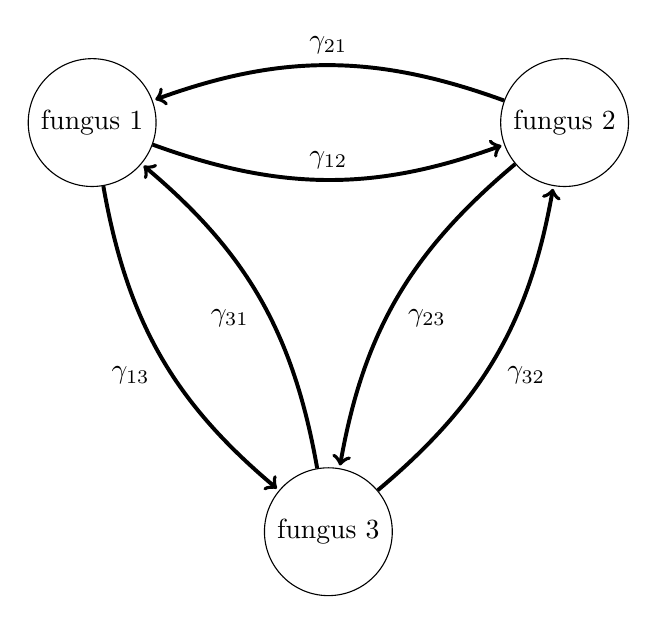
\begin{tikzpicture}
            \node[draw, circle] at (0, 0)     (1)     {fungus 1};
            \node[draw, circle] at (6, 0)     (2)     {fungus 2};
            \node[draw, circle] at (3, -5.196) (3) {fungus 3};
    
            \draw[every loop, auto=right, line width=0.5mm]
                (1) edge[bend right=20]            node {$\gamma_{13}$} (3)
                (1) edge[bend right=20, auto=left] node {$\gamma_{12}$} (2)
                (2) edge[bend right=20]            node {$\gamma_{21}$} (1)
                (2) edge[bend right=20, auto=left] node {$\gamma_{23}$} (3)
                (3) edge[bend right=20]            node {$\gamma_{32}$} (2)
                (3) edge[bend right=20, auto=left] node {$\gamma_{31}$} (1);
        \end{tikzpicture}
    \end{center}
\end{figure}


\subsection{Constructing Markov chain for fungus community}

Consider a given time interval $T$, and the population density of each fungus species at time $t$ is denoted as $\boldsymbol{x}(t) = [x_1(t), x_2(t), \cdots, x_n(t)]^T$. In the evolution process of the community, at each time interval, a specific percentage of fungi $i$ is remained, and others can be considered as transformed into population density of other species of fungus.

For a simple dual-species system, such transition relation can be expressed as

% TODO: Redefine the matrix

\begin{equation}
    \left\{\begin{aligned} &
        x_1(t+T) = \gamma_{11}x_1(t) + \gamma_{21}x_2(t) \\ &
        x_2(t+T) = \gamma_{22}x_2(t) + \gamma_{12}x_1(t)
    \end{aligned}\right..
\end{equation}

More generally, in an $n$-species community, the system is characterized by

\begin{equation}
    \left\{\begin{aligned} &
        x_1(t+T) = \gamma_{11}x_1(t) + \cdots + \gamma_{n1}x_n(t) \\ & \cdots \\ &
        x_i(t+T) = \sum_{j=1}^n \gamma_{ij}x_j \\ & \cdots \\ &
        x_n(t+T) = \gamma_{n1}x_1(t) + \cdots + \gamma_{nn}x_n(t).
    \end{aligned}\right.
\end{equation}

Which can be further simplified with matrix notation.

\begin{equation}\label{eq:trans}
    \boldsymbol{x}(t+T) = \boldsymbol{Y}\boldsymbol{x}(t).
\end{equation}

In which, the matrix $\boldsymbol{Y}_{n\times n}$ is defined to be the transition matrix of the system, with element $\gamma_{ij}$ denoting the transition rate from fungus specie $i$ to $j$.

\begin{equation}
    \boldsymbol{Y} =
    \begin{bmatrix}
        \gamma_{11} & \gamma_{12} & \cdots & \gamma_{1n} \\
        \gamma_{21} & \ddots & & \vdots \\
        \vdots & & \ddots & \vdots \\
        \gamma_{n1} & \cdots & \cdots & \gamma_{nn}
    \end{bmatrix}
\end{equation}

Note that the transition rate in the biological configuration considerably differs from that in stochastic process. In a typical Markov chain model, each element in the transition matrix represents a certain probability of transition or decision towards another state. To implement this model in a continuous mathematical configuration, adjustments must be and evidently can be made to the definition of the population density $x_i$ itself, ensuring that a unit of population density of different species of fungus takes up the same amount of resources in the system. With such adjustment, it is guaranteed that, for each element and row of the transition matrix, we have

\begin{equation}\label{eq:markov-norm}
    \left\{\begin{aligned} &
        \boldsymbol{Y}_{ij} \in [0,\ 1],\ i,\ j\in\{1,\ 2,\ \cdots,\ n\} \\ &
        \sum_{j=1}^n \boldsymbol{Y}_{ij} = 1,\ i\in\{1,\ 2,\ \cdots,\ n\}.
    \end{aligned}\right.
\end{equation}

In addition, though during the growth process of the populations, and in macroscopic view the early stage of the decomposition, the transition matrix may not satisfy condition \eqref{eq:markov-norm}, and the sum of the rows could possibly even vary with time, it is shown that the final homeostasis is only related to the transition matrix after the community enters Markov process.


\subsection{Incorporate hyphal extension rate and moisture tolerance}

To model the system of fungi community, the transition matrix is further specified as follows in order to incorporate traits we concerned.

\begin{equation}\label{eq:gamma}
    \gamma_{ij} = \frac{r_i/r_j}{\sum_{k=1}^n r_i/r_k}.
\end{equation}

The hyphal extension rate is a significant trait characterizing the \textbf{combative ability} of fungus, the ratio represents how combative a fungus can be when replacing another fungus isolate. It can be easily verified that, definition \eqref{eq:gamma} is normalized for keeping consistent with prerequisite \eqref{eq:markov-norm}.

\subsection{The homeostasis of the system}

% Once the total population density reached the overall carrying capacity of the system, condition \eqref{eq:norm} is automatically satisfied. It is obvious that, according to \eqref{eq:trans}, after $nT$ time, the the population density in the community turns into

% \begin{equation}
%     \boldsymbol{x}(t+nT) =
%     \boldsymbol{Y}\boldsymbol{x}[t+(n-1)T] = \cdots =
%     \boldsymbol{Y}^n\boldsymbol{x}(t).
% \end{equation}

% For solving this model, consider the eigenvalues and eigenvectors of the transition matrix\dots

% \begin{equation}
%     \boldsymbol{Y}\boldsymbol{z} = \lambda\boldsymbol{z} \Rightarrow
% \end{equation}

In a Markov process, the final homeostasis is only related to the transition matrix, but cannot be explicitly expressed.

We postulate a quad-species fungi community, among them two in the top and two in the bottom of the competitive ranking, to visualize and verify this model.

\begin{table}\caption{The four species chosen in verifying the model}
    \centering
    \begin{tabular}{ccc}
        \toprule
        Specie & Competitive Ranking & Hyphal Extension Rate \\
        \midrule
        Phlebia acerina MR4280 B9G & 1 & 8.75 \\
        Phlebiopsis flavidoalba FP150451 A8G & 0.9864 & 10.8 \\
        Armillaria gallica HHB12551 C6C & 0 & 0.49 \\
        Armillaria tabescens TJV93 261 A1E & 0 & 1.07 \\
        \bottomrule
    \end{tabular}
\end{table}

% TODO: Give example

\section{Solution and Result}\label{sec:solu}


\section{Analysis}\label{sec:analysis}

\subsection{Sensitivity Analysis}


\subsection{Strengths and Weaknesses}

\section{Conclusions}\label{sec:conclu}

In conclusion, hyphal extension rate and moisture tolerance are positively related to the decay ability of a fungi isolate as well as the community. In a fungi community, the decay ability is determined by its community-weighted hyphal extension rate. The composition of a fungi community in homeostasis can be inferred from Markov chain model or solving adaptive LV-model.

Environmental conditions have affect on the composition of the community, hence alters the decay ability. The larger the varying range of local environmental condition is, the slower the decomposition becomes. Certain species combinations may suitably persis in corresponding climate. In general, biodiversity is positively related to the decay ability.

\section{Future Works}\label{sec:future}



\section*{Competition, Adaptation and Diversity: How Fungi Support Our Biosphere}

\setcounter{figure}{0}

Fungi are everywhere in the world, not just on a rotten orange, or in yeast essential bread and cake. Fungi together with a series of other microbes plays an important role in the biosphere, know as the \textbf{decomposers}. The normal functionality of biosphere requires both sustained energy and material flow, and the latter one consists of not only essential organic chemical compound such as amino acids and glucose, but also inorganic carbon dioxide. Such material flow is also called the \textbf{carbon cycle}\dots

\begin{figure}[ht]
    \centering
    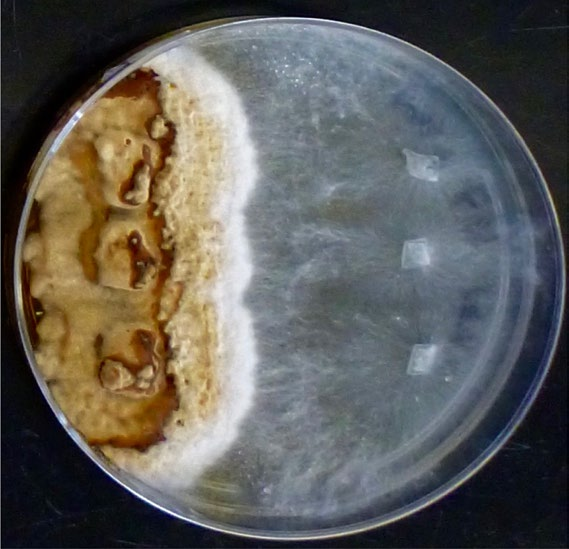
\includegraphics[width=0.4\textwidth]{isolate.jpg}
    \caption{Fungi in pair wise competition test. This figure is adopted from ``Consistent trade-offs in fungal trait expression across broad spatial scales" by Daniel S. Maynard et al.}
    \label{fig:decom-hyphal-122d}
\end{figure}

In carbon cycle, the \textbf{producers}, mainly the green plants, are responsible for the fixation of carbon, namely transforming the carbon in carbon dioxide into fixed carbon in organic matter through chemosynthesis, of which the most commonly known one is photosynthesis. Then, the \textbf{consumers} utilize these material for vital activities, some carbon transformed into again into the carbon dioxide, some maintain in consumers.

What would these carbon go? Can they go back to the atmosphere? This is where decomposers play a role. Decomposers decompose the cadavers and excrements, function as the bridge in the carbon cycle. Note that, one of the most important features of carbon cycle is that it was global, the beef, egg and milk consumptions in the US might be related to the depletion of Brazilian rain forests, which is why carbon cycle is significant to us all and more and more researchers are interested in this topic.

As an important category in decomposers, fungi are outstanding participants in the decay process, especially when dealing with ground litter and woody fibers. A recent research presented the mechanism of decay efficiency for fungi community. The decay ability is positively related to the hyphal extension rate and moisture tolerance of a fungus isolate. However, as for a fungi community, the thing is getting more complicated.

\begin{figure}
    \centering
    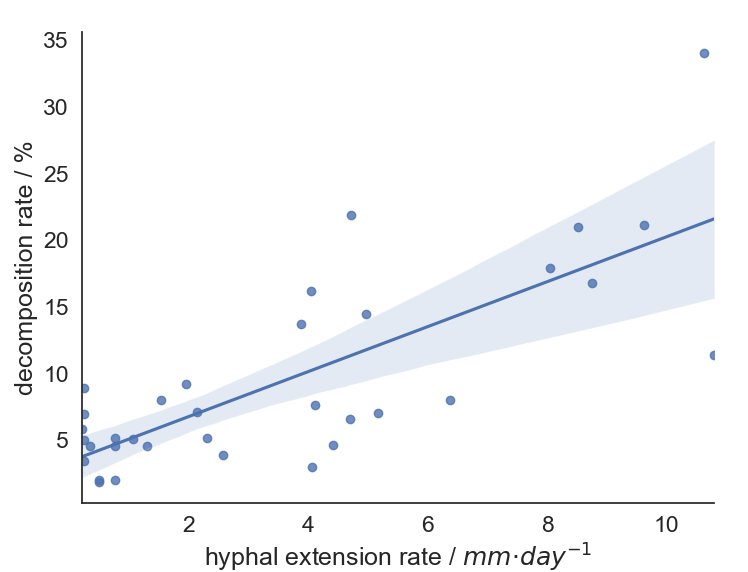
\includegraphics[width=0.6\textwidth]{decom-hyphal-122d.png}
    \caption{The relationship between the hyphal extension rate of various fungi and the resulting wood decomposition rate. The hyphal extension rate is the geometrical average of the value tested under 10, 16 and 22 Celsius.}
\end{figure}

The composition of the fungi community can be predicted by the famous Lotka-Volterra model as shown in \eqref{eq:lv}, which indicates that in a multi-species system, each species would exert stress on other species. Tilman interprets that, the intrinsic mechanism is the limitation of certain resources. Generally, the fungus which grows slower, can better tolerate a wide range of environmental conditions. Therefore, some most competitive fungi may attain huge superiority at the start, and replace the less combative fungi completely. Sometime, more tolerant fungi might be able to endure the oppression and gain dominance in the later stages. Such feature determines that, some combinations of fungi may be able to persist and reach a dynamic homeostasis. It is apparent that, these combinations may vary with environmental conditions, you may do your own experiments in the laboratory to find out the ``recipe".

\[
    \label{eq:lv}\tag{$\ast$}
    \frac{\mathrm{d}x_i}{\mathrm{d}t} =
    r_ix_i\left(1 - \frac{\sum_{j=1}^n \alpha_{ij}x_j}{K_i}\right)
\]

Another interesting fact is that, when less competitive species of fungi are introduced to the community, the decay ability of the fungi community may be boosted instead of decreased. This phenomenon can be explained as, different species are preponderant in decomposing at different stages. A large varieties of species, namely the \textbf{biodiversity}, enables the possibility of various combinations. Such combination is relevant to the climatic conditions, resulting unique biodiversity in different geographical areas.

The global carbon cycle integrates whole biosphere all together, with inconspicuous fungi as a crucial part in it. It is our shared responsibility to restrict carbon emission and protect biodiversity. Hope next time you could feel less disgusted when seeing a rotten apple, it might be fungi answering their call!


% References
\newpage
\bibliographystyle{unsrt}
\bibliography{biblo}
\newpage


% Appendix 
\appendixpage
\appendix

\section{Source Code}

The source code for Markov chain model.

\inputminted[linenos=true, frame=single]{python}{codes/appendix.py}


\section{Fungi Traits Data}

The decomposition rate data from \cite{Lustenshouwer}, can be retrieved at \href{https://www.pnas.org/content/pnas/suppl/2020/05/13/1909166117.DCSupplemental/pnas.1909166117.sapp.pdf}{Supplementary Information for A trait-based understanding of wood decomposition by fungi}.

The other fungi traits data from \cite{Maynard-data}, can be retrieved at \href{https://github.com/dsmaynard/fungal_biogeography}{dsmaynard/fungal\_biogeography}.


\end{document}

